\documentclass[12pt]{article}\usepackage[]{graphicx}\usepackage[]{color}
%% maxwidth is the original width if it is less than linewidth
%% otherwise use linewidth (to make sure the graphics do not exceed the margin)
\makeatletter
\def\maxwidth{ %
  \ifdim\Gin@nat@width>\linewidth
    \linewidth
  \else
    \Gin@nat@width
  \fi
}
\makeatother

\definecolor{fgcolor}{rgb}{0.345, 0.345, 0.345}
\newcommand{\hlnum}[1]{\textcolor[rgb]{0.686,0.059,0.569}{#1}}%
\newcommand{\hlstr}[1]{\textcolor[rgb]{0.192,0.494,0.8}{#1}}%
\newcommand{\hlcom}[1]{\textcolor[rgb]{0.678,0.584,0.686}{\textit{#1}}}%
\newcommand{\hlopt}[1]{\textcolor[rgb]{0,0,0}{#1}}%
\newcommand{\hlstd}[1]{\textcolor[rgb]{0.345,0.345,0.345}{#1}}%
\newcommand{\hlkwa}[1]{\textcolor[rgb]{0.161,0.373,0.58}{\textbf{#1}}}%
\newcommand{\hlkwb}[1]{\textcolor[rgb]{0.69,0.353,0.396}{#1}}%
\newcommand{\hlkwc}[1]{\textcolor[rgb]{0.333,0.667,0.333}{#1}}%
\newcommand{\hlkwd}[1]{\textcolor[rgb]{0.737,0.353,0.396}{\textbf{#1}}}%

\usepackage{framed}
\makeatletter
\newenvironment{kframe}{%
 \def\at@end@of@kframe{}%
 \ifinner\ifhmode%
  \def\at@end@of@kframe{\end{minipage}}%
  \begin{minipage}{\columnwidth}%
 \fi\fi%
 \def\FrameCommand##1{\hskip\@totalleftmargin \hskip-\fboxsep
 \colorbox{shadecolor}{##1}\hskip-\fboxsep
     % There is no \\@totalrightmargin, so:
     \hskip-\linewidth \hskip-\@totalleftmargin \hskip\columnwidth}%
 \MakeFramed {\advance\hsize-\width
   \@totalleftmargin\z@ \linewidth\hsize
   \@setminipage}}%
 {\par\unskip\endMakeFramed%
 \at@end@of@kframe}
\makeatother

\definecolor{shadecolor}{rgb}{.97, .97, .97}
\definecolor{messagecolor}{rgb}{0, 0, 0}
\definecolor{warningcolor}{rgb}{1, 0, 1}
\definecolor{errorcolor}{rgb}{1, 0, 0}
\newenvironment{knitrout}{}{} % an empty environment to be redefined in TeX

\usepackage{alltt}
\usepackage[top=1in, bottom= 1in, left= 1in, right= 1in]{geometry}
\usepackage[USenglish]{babel} % set the language; greek allows \textgreek{\euro}
\usepackage{multirow} % For tables
\usepackage{graphicx, subfigure} % For graphics
\usepackage{fancyhdr} % Produces fancy headers
\usepackage{setspace} % allows for vsape
\usepackage{natbib} % package to organize literature --> google it!
\usepackage{verbatim} % For including R-code
\usepackage{booktabs} % nicer tables
\usepackage{alltt} % verbatim + highlighting
\usepackage{amsmath} %boldsymbols
\usepackage{lscape} %Querformat
\usepackage{dcolumn} % align at decimal mark
\usepackage{floatrow} % description paragraphs below figures and tables
\usepackage{enumerate} % alter enumerate items (i,ii,iii etc)
\usepackage[colorlinks=true,citecolor=blue,urlcolor=blue]{hyperref}
\setlength{\headheight}{15pt}
% http://en.wikibooks.org/wiki/LaTeX/Page_Layout for additional info

\title{Comparison of the Efficiency of Majority Election Results}
\author{}
\IfFileExists{upquote.sty}{\usepackage{upquote}}{}

\begin{document}
\maketitle

\section*{Overview of Simulation Parameters}
\begin{itemize}
\item Number of simulations for each scenario: 1000
\item Numbers of voters: 10, 20, 50, 100, 200, 500, 1000, 2000, 5000, 10000
\item Utility distributions for each voter (candidates $A$ and $B$): \\
$\begin{pmatrix}U_A\\ U_B \end{pmatrix} \sim \mathcal{N}\left(
\boldsymbol{\mu}=\begin{pmatrix}0+\epsilon \\ 0-\epsilon \end{pmatrix},
\mathbf{\Sigma}=\begin{pmatrix}1 & \sigma^2 \\ \sigma^2 & 1\end{pmatrix}\right)$
\item Differences in distribution means ($\epsilon$): 0, 0.005, 0.01, 0.025, 0.05, 0.1, 0.25, 0.5, 0.75, 1
\item Correlations between utilities ($\sigma^2$): 0, 0.9, -0.9
\item Skewness of distribution ($\alpha$): 0, 10, -10 

\end{itemize}




\clearpage
\section{Normally Distributed Utilities (no skewness)}
\begin{knitrout}
\definecolor{shadecolor}{rgb}{0.969, 0.969, 0.969}\color{fgcolor}
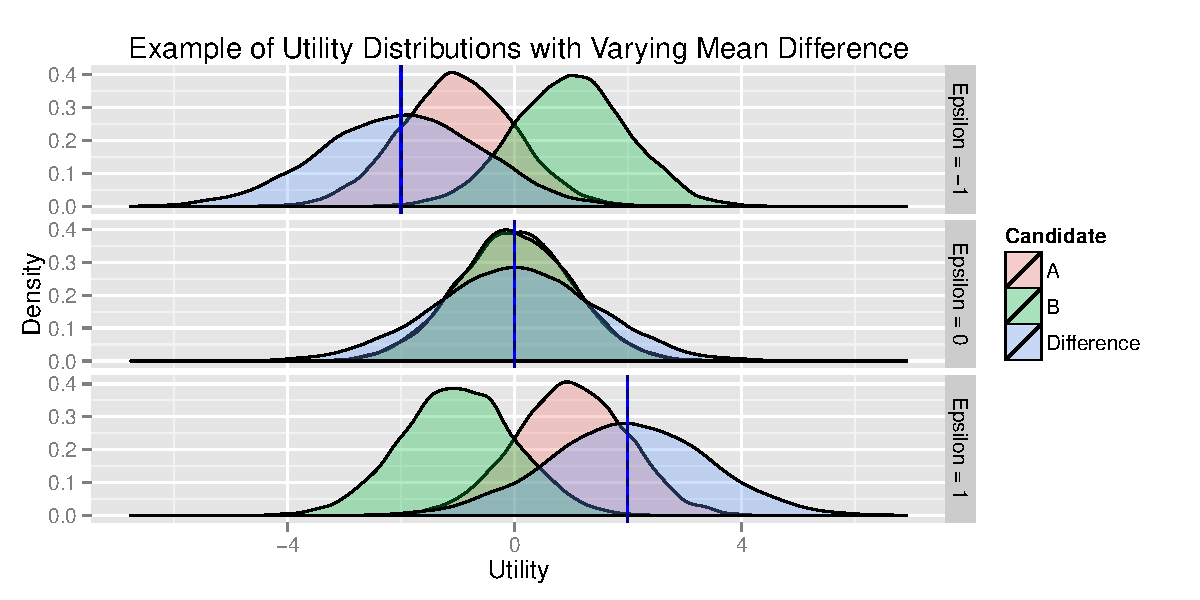
\includegraphics[width=\maxwidth]{figure/unnamed-chunk-2} 

\end{knitrout}


\subsection{No Correlation Between Utilities}
\begin{knitrout}
\definecolor{shadecolor}{rgb}{0.969, 0.969, 0.969}\color{fgcolor}
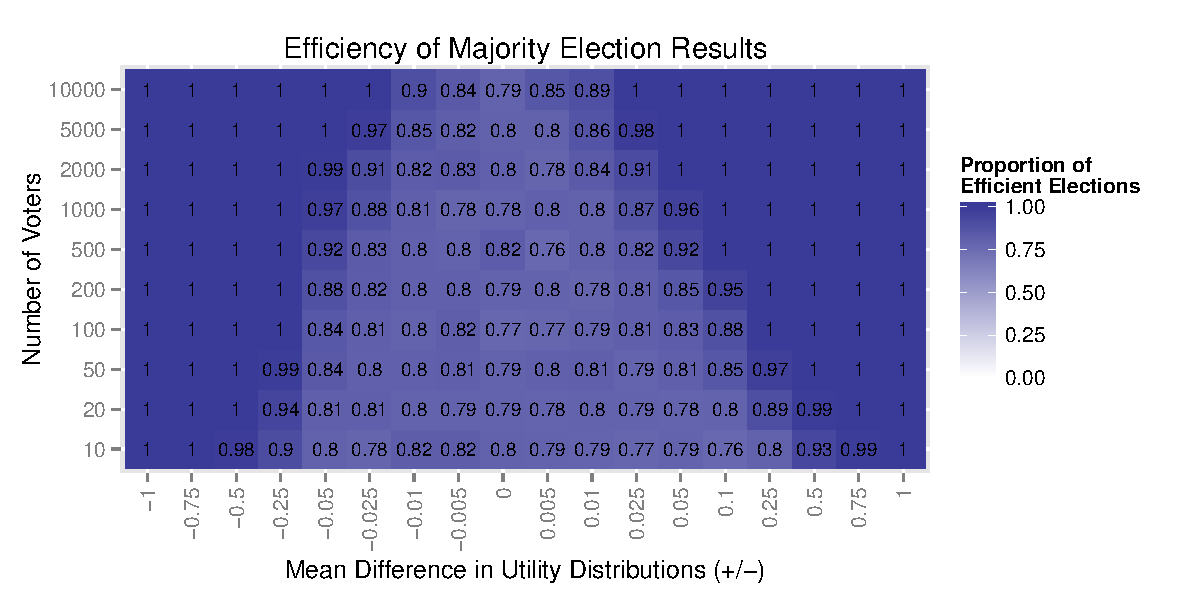
\includegraphics[width=\maxwidth]{figure/unnamed-chunk-3} 

\end{knitrout}


\clearpage
\subsection{Positive Correlation Between Utilities}
\begin{knitrout}
\definecolor{shadecolor}{rgb}{0.969, 0.969, 0.969}\color{fgcolor}
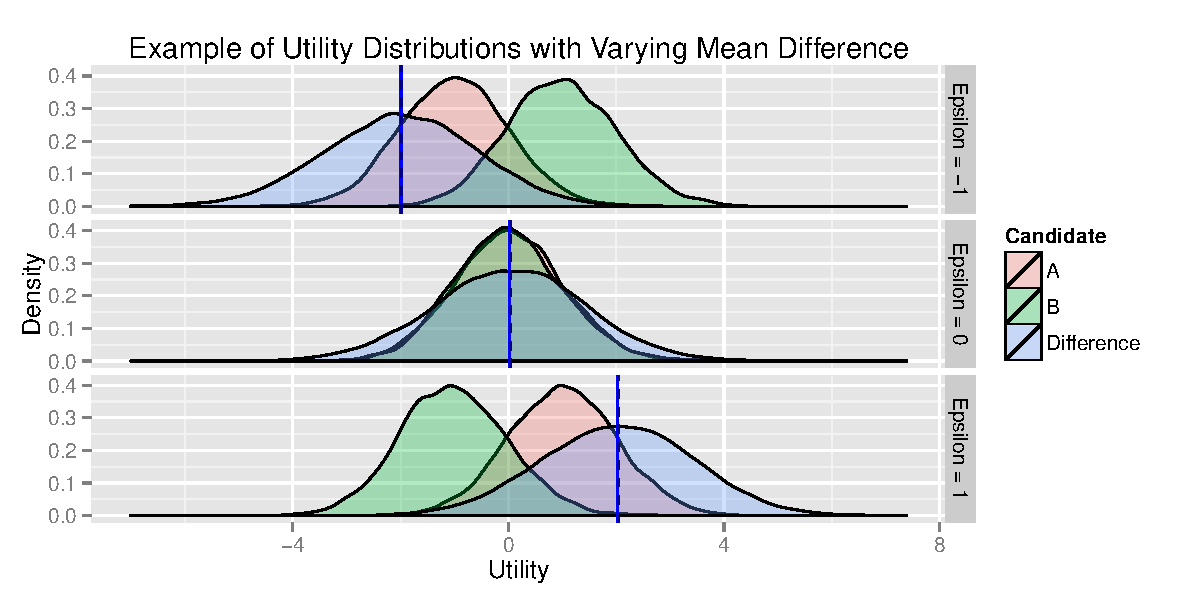
\includegraphics[width=\maxwidth]{figure/unnamed-chunk-4} 

\end{knitrout}


\subsection{Negative Correlation Between Utilities}
\begin{knitrout}
\definecolor{shadecolor}{rgb}{0.969, 0.969, 0.969}\color{fgcolor}
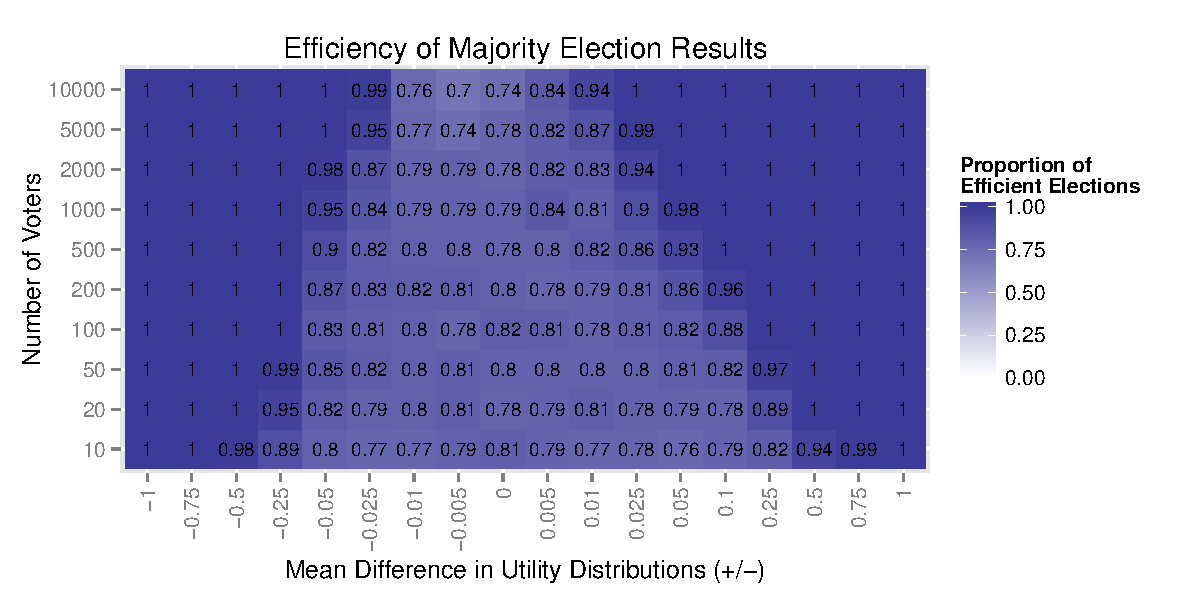
\includegraphics[width=\maxwidth]{figure/unnamed-chunk-5} 

\end{knitrout}



\section{Positively Skewed Utilities}
\begin{knitrout}
\definecolor{shadecolor}{rgb}{0.969, 0.969, 0.969}\color{fgcolor}
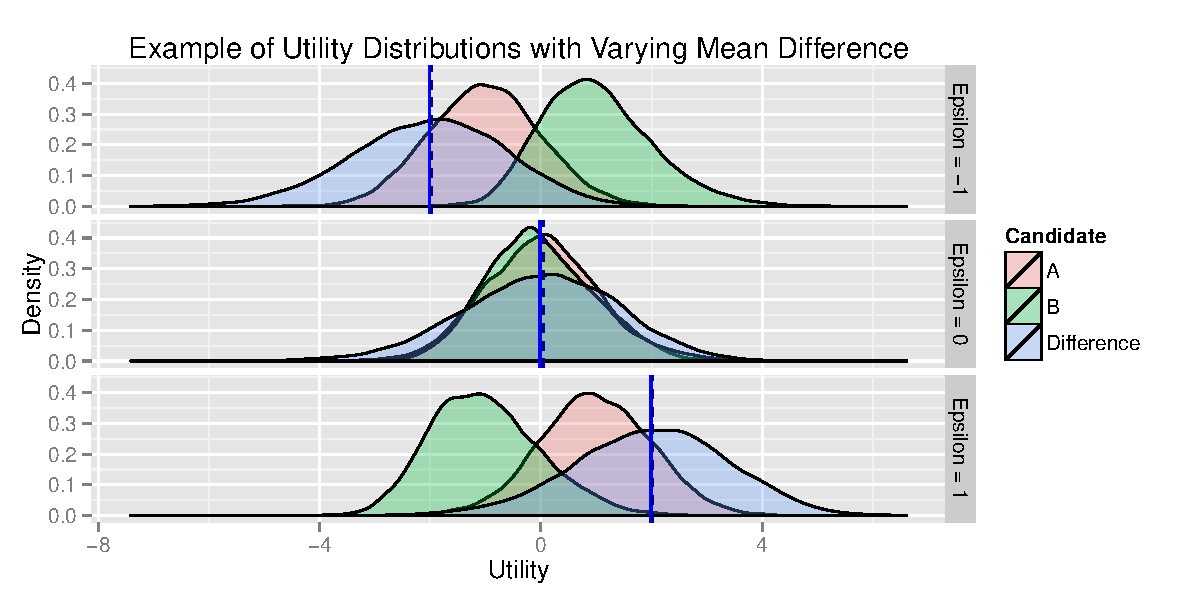
\includegraphics[width=\maxwidth]{figure/unnamed-chunk-6} 

\end{knitrout}


\subsection{No Correlation Between Utilities}
\begin{knitrout}
\definecolor{shadecolor}{rgb}{0.969, 0.969, 0.969}\color{fgcolor}
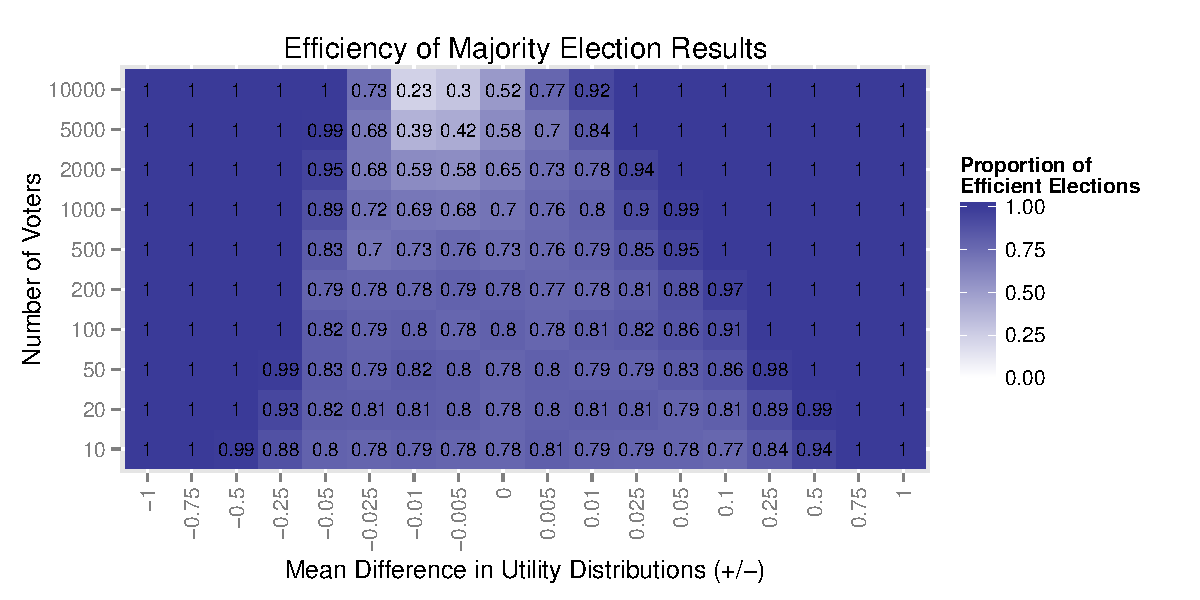
\includegraphics[width=\maxwidth]{figure/unnamed-chunk-7} 

\end{knitrout}


\clearpage
\subsection{Positive Correlation Between Utilities}
\begin{knitrout}
\definecolor{shadecolor}{rgb}{0.969, 0.969, 0.969}\color{fgcolor}
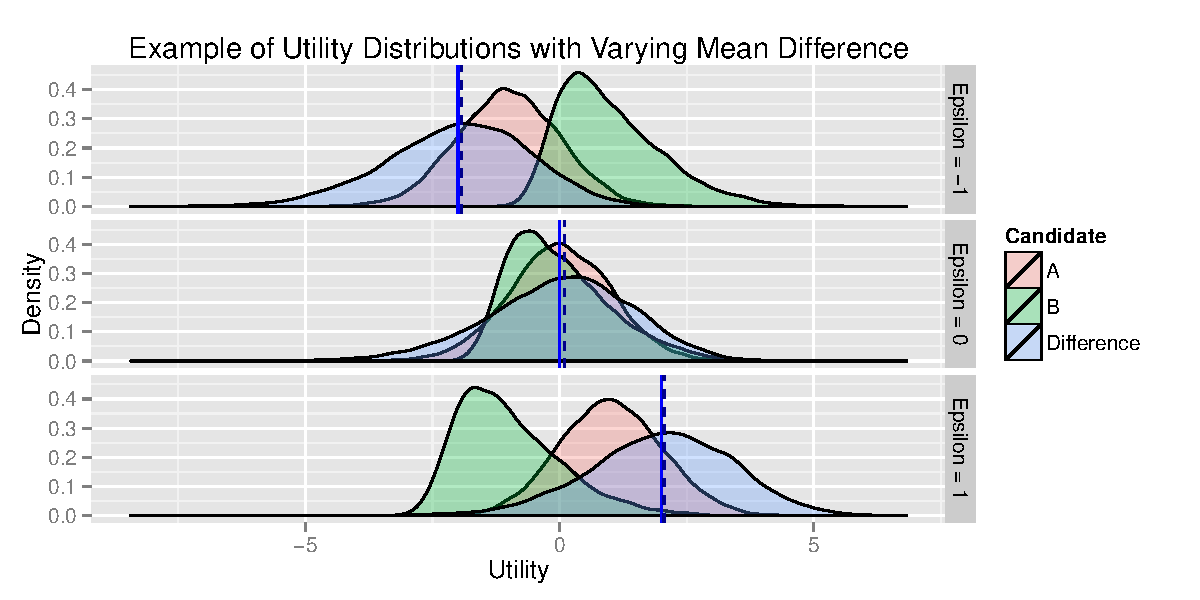
\includegraphics[width=\maxwidth]{figure/unnamed-chunk-8} 

\end{knitrout}


\subsection{Negative Correlation Between Utilities}
\begin{knitrout}
\definecolor{shadecolor}{rgb}{0.969, 0.969, 0.969}\color{fgcolor}
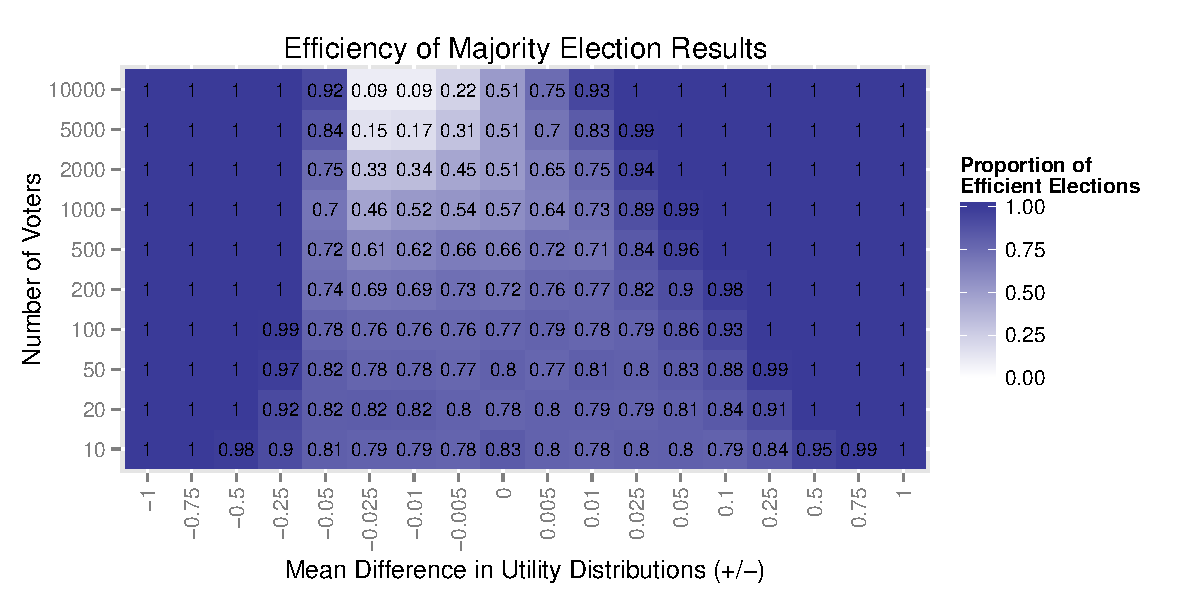
\includegraphics[width=\maxwidth]{figure/unnamed-chunk-9} 

\end{knitrout}



\section{Negatively Skewed Utilities}
\begin{knitrout}
\definecolor{shadecolor}{rgb}{0.969, 0.969, 0.969}\color{fgcolor}
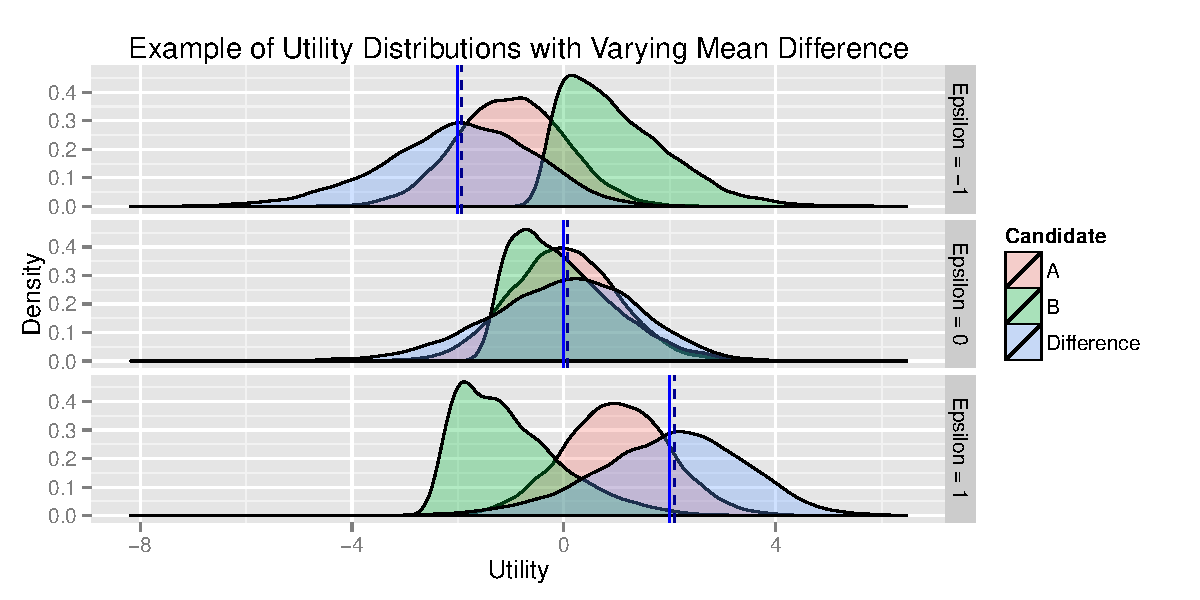
\includegraphics[width=\maxwidth]{figure/unnamed-chunk-10} 

\end{knitrout}


\subsection{No Correlation Between Utilities}
\begin{knitrout}
\definecolor{shadecolor}{rgb}{0.969, 0.969, 0.969}\color{fgcolor}
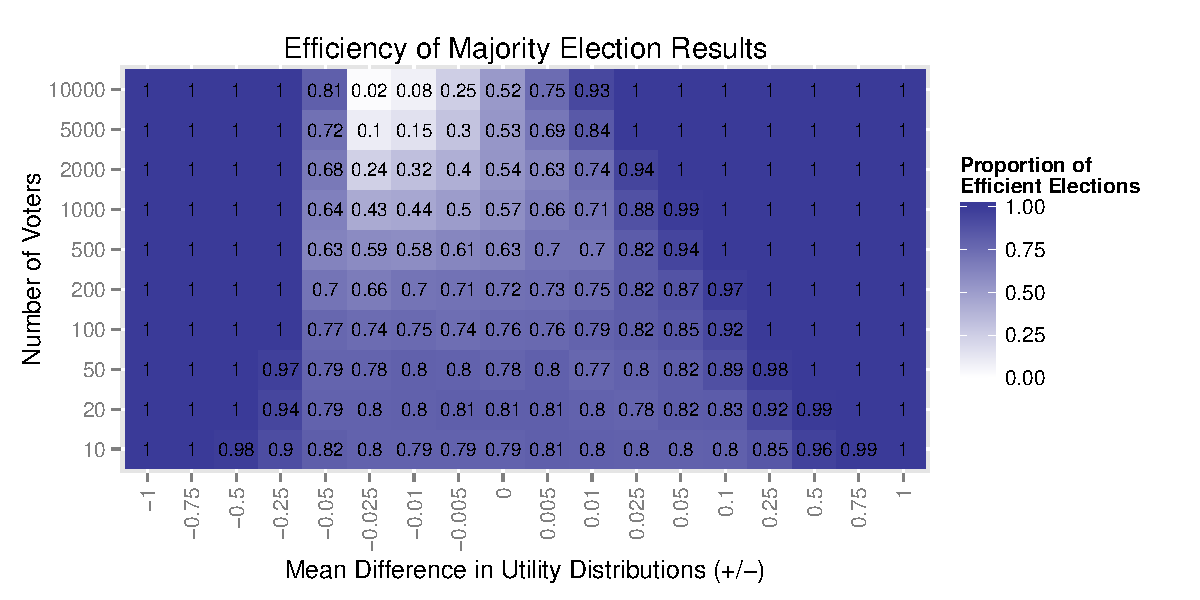
\includegraphics[width=\maxwidth]{figure/unnamed-chunk-11} 

\end{knitrout}


\clearpage
\subsection{Positive Correlation Between Utilities}
\begin{knitrout}
\definecolor{shadecolor}{rgb}{0.969, 0.969, 0.969}\color{fgcolor}
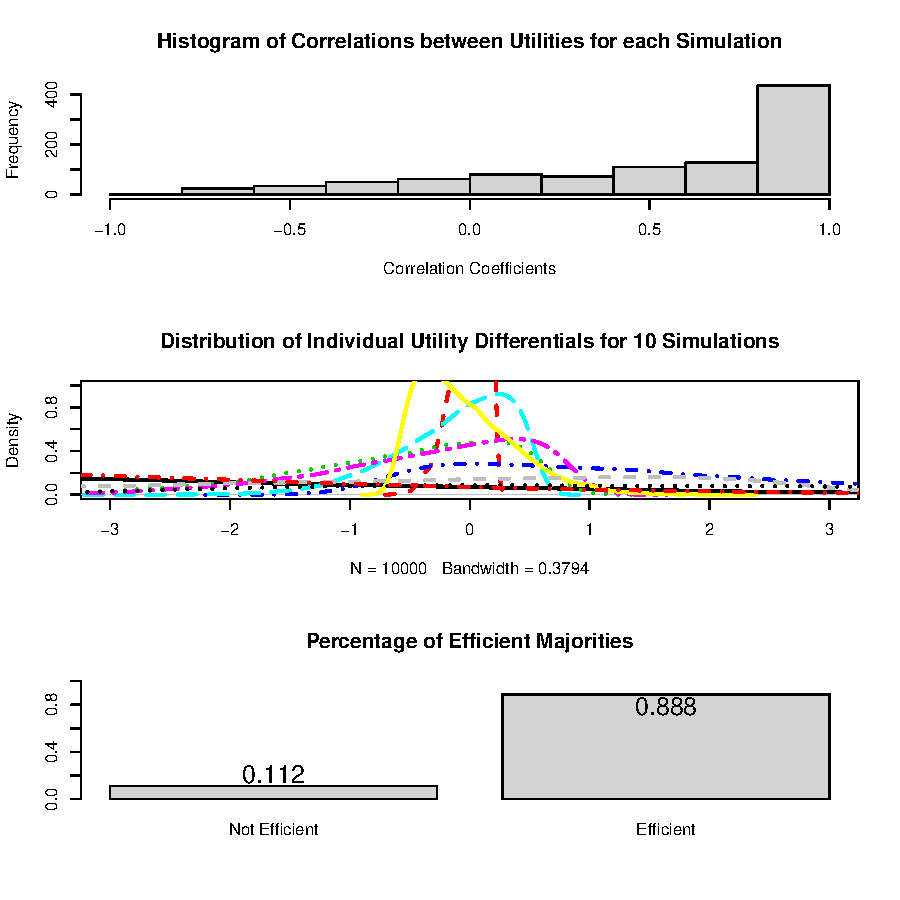
\includegraphics[width=\maxwidth]{figure/unnamed-chunk-12} 

\end{knitrout}


\subsection{Negative Correlation Between Utilities}
\begin{knitrout}
\definecolor{shadecolor}{rgb}{0.969, 0.969, 0.969}\color{fgcolor}
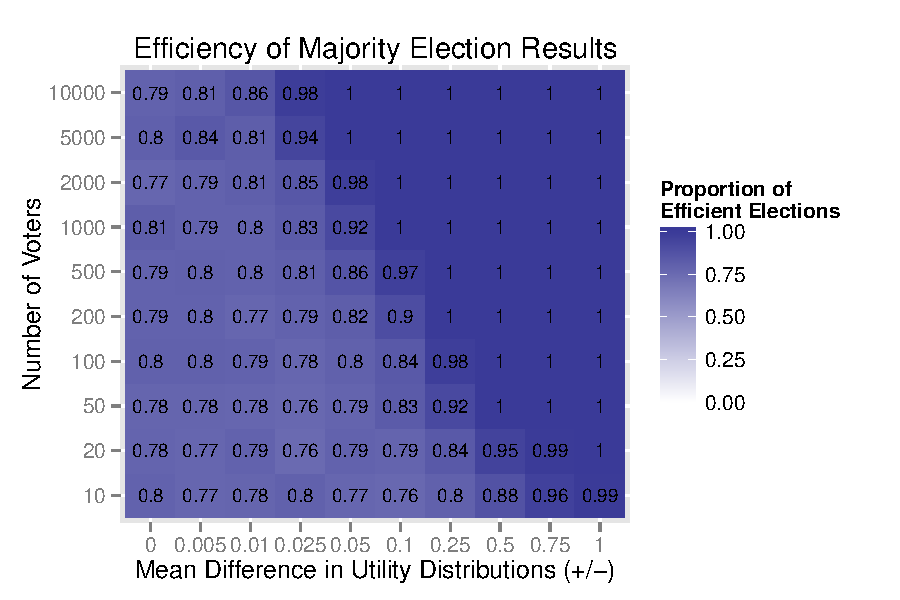
\includegraphics[width=\maxwidth]{figure/unnamed-chunk-13} 

\end{knitrout}



\section{Utilities with Opposing Skewness: Positive Skew for Favored Candidate}
\begin{knitrout}
\definecolor{shadecolor}{rgb}{0.969, 0.969, 0.969}\color{fgcolor}
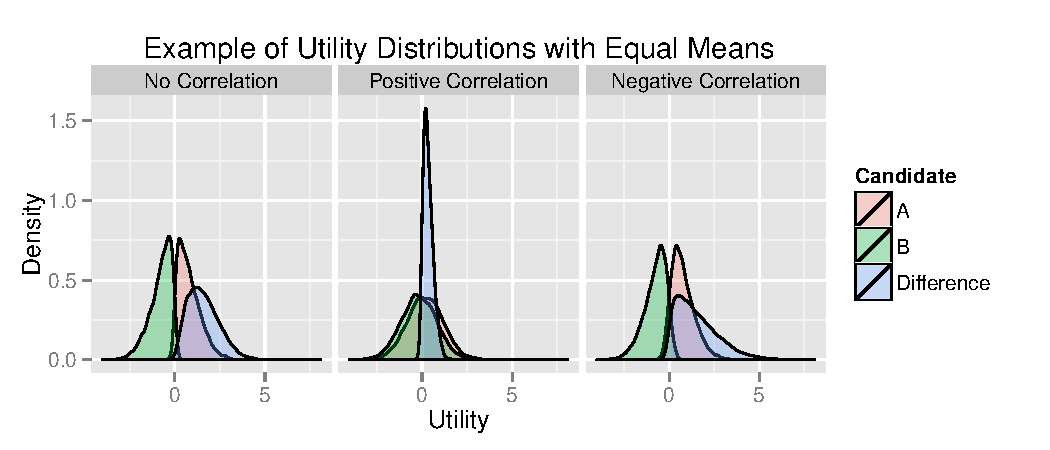
\includegraphics[width=\maxwidth]{figure/unnamed-chunk-14} 

\end{knitrout}


\subsection{No Correlation Between Utilities}
\begin{knitrout}
\definecolor{shadecolor}{rgb}{0.969, 0.969, 0.969}\color{fgcolor}
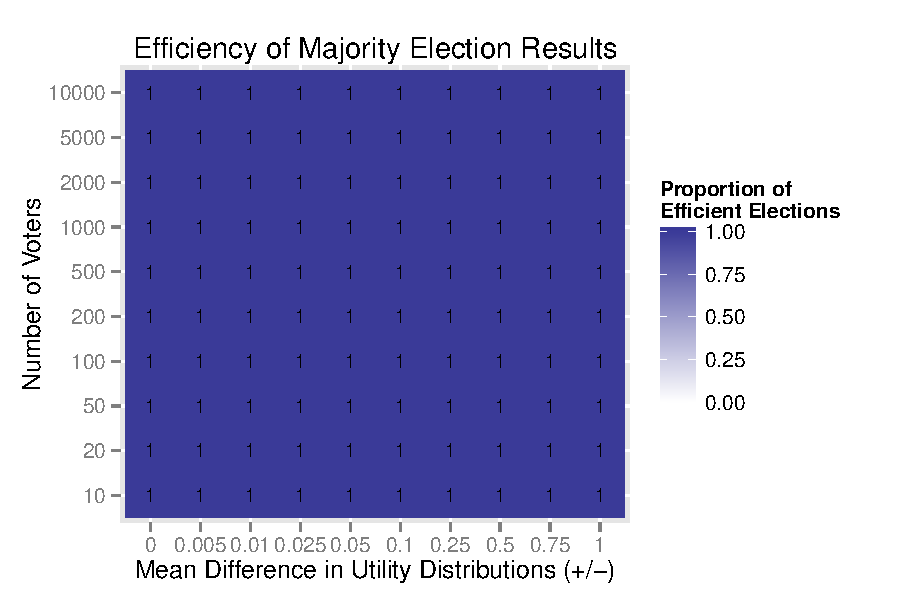
\includegraphics[width=\maxwidth]{figure/unnamed-chunk-15} 

\end{knitrout}


\clearpage
\subsection{Positive Correlation Between Utilities}
\begin{knitrout}
\definecolor{shadecolor}{rgb}{0.969, 0.969, 0.969}\color{fgcolor}
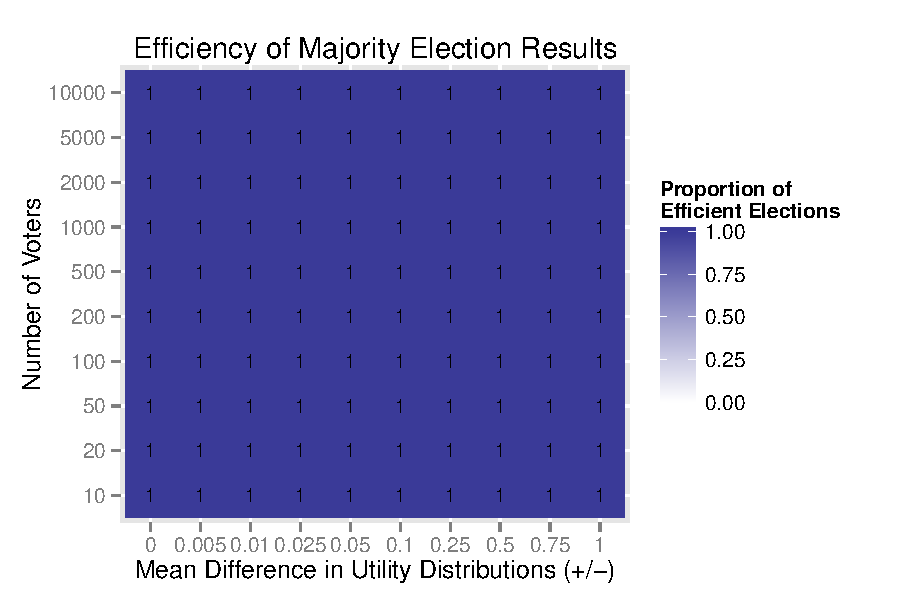
\includegraphics[width=\maxwidth]{figure/unnamed-chunk-16} 

\end{knitrout}


\subsection{Negative Correlation Between Utilities}
\begin{knitrout}
\definecolor{shadecolor}{rgb}{0.969, 0.969, 0.969}\color{fgcolor}
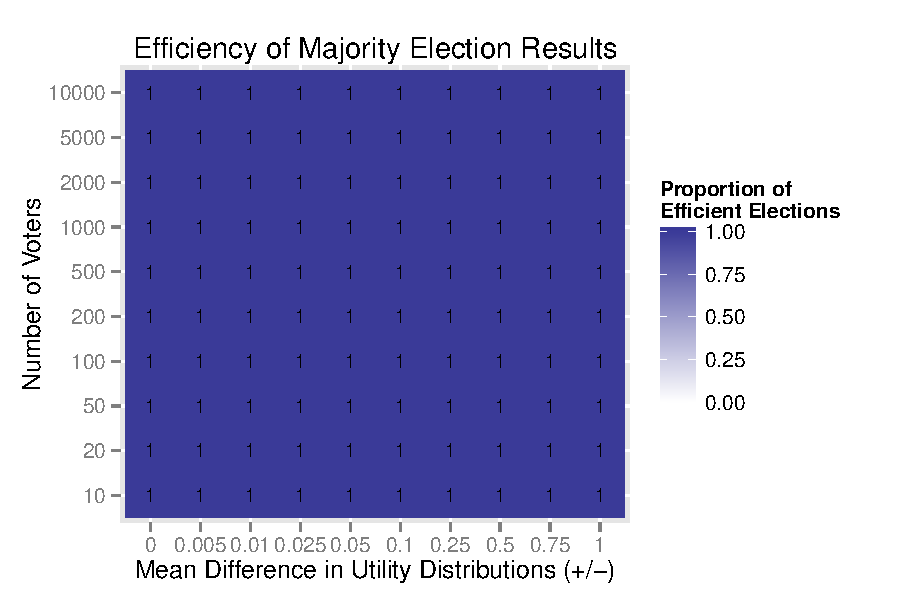
\includegraphics[width=\maxwidth]{figure/unnamed-chunk-17} 

\end{knitrout}



\section{Utilities with Opposing Skewness: Negative Skew for Favored Candidate}
\begin{knitrout}
\definecolor{shadecolor}{rgb}{0.969, 0.969, 0.969}\color{fgcolor}
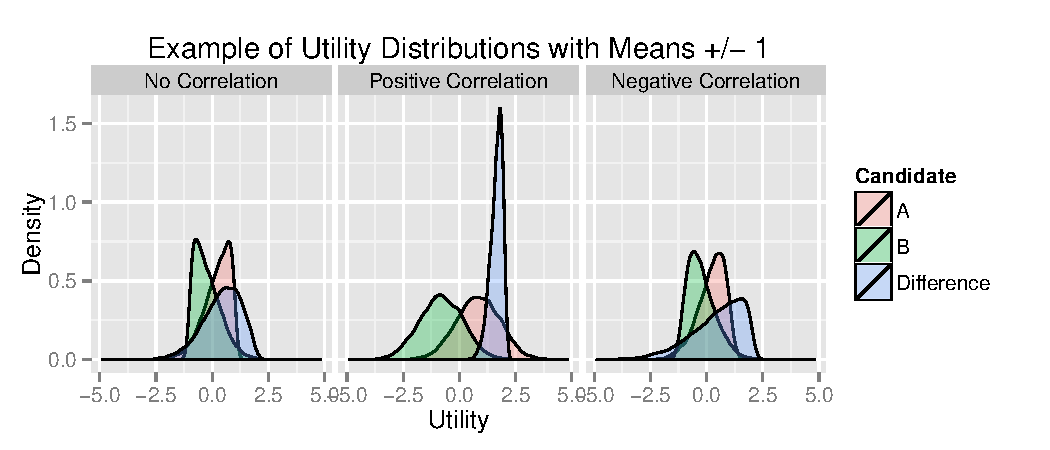
\includegraphics[width=\maxwidth]{figure/unnamed-chunk-18} 

\end{knitrout}


\subsection{No Correlation Between Utilities}
\begin{knitrout}
\definecolor{shadecolor}{rgb}{0.969, 0.969, 0.969}\color{fgcolor}
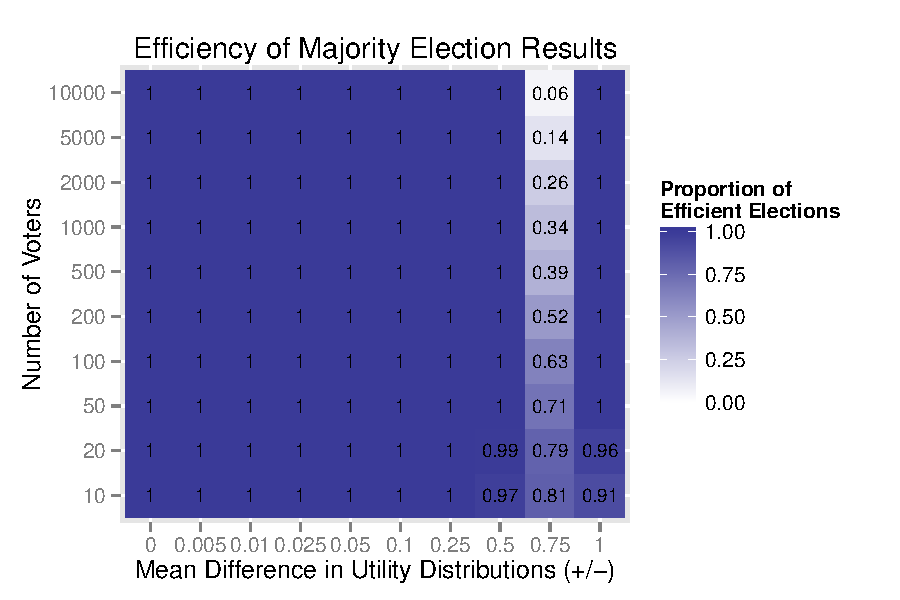
\includegraphics[width=\maxwidth]{figure/unnamed-chunk-19} 

\end{knitrout}


\clearpage
\subsection{Positive Correlation Between Utilities}
\begin{knitrout}
\definecolor{shadecolor}{rgb}{0.969, 0.969, 0.969}\color{fgcolor}
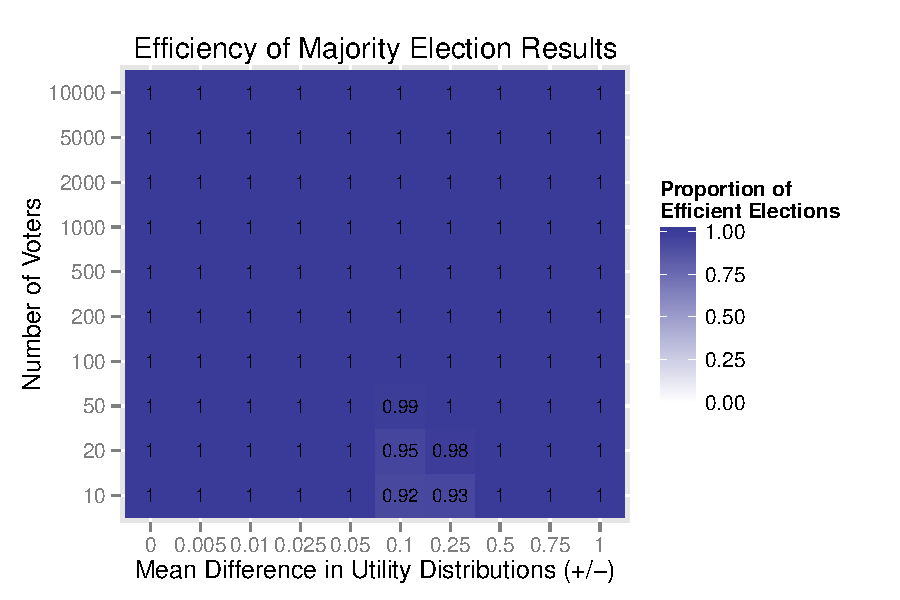
\includegraphics[width=\maxwidth]{figure/unnamed-chunk-20} 

\end{knitrout}


\subsection{Negative Correlation Between Utilities}
\begin{knitrout}
\definecolor{shadecolor}{rgb}{0.969, 0.969, 0.969}\color{fgcolor}
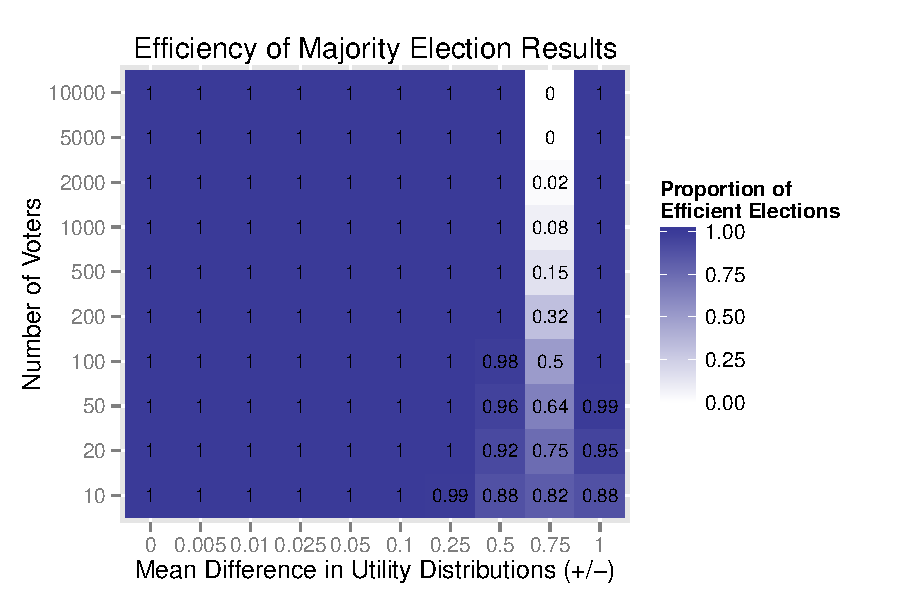
\includegraphics[width=\maxwidth]{figure/unnamed-chunk-21} 

\end{knitrout}



\end{document}
